% !TEX program = lualatex

\documentclass[
11pt,
captions=tableheading,
smallheadings,
%headings=big,
headsepline,
footsepline, 
%chapterprefix=false			% weiss nicht was passiert
captions=tableheading,
parskip=half-,
%BCOR=10mm,
%twocolumn, 
%draft
]{scrartcl}

%\usepackage[babelshorthands]{polyglossia}
\usepackage{polyglossia}
\setdefaultlanguage[variant = swiss]{german}

%\usepackage[ngerman]{babel}

%\usepackage[ngerman]{babel} 
\usepackage[]{ scrlayer-scrpage }
\usepackage[ a4paper,
 total={165mm,244mm},
 left=25mm,
 top=25mm,
 headsep=10mm
 %footsep=12mm
 %,showframe
  ]{geometry}
 \usepackage{fontspec}
\setmainfont{Times New Roman}
\setsansfont{Arial}

\usepackage[dvipsnames]{xcolor}
\usepackage[most]{tcolorbox}
\usepackage[
version=3,
arrows=pgf-filled,
]{mhchem} % für chemische Formeln
\usepackage{microtype}
\usepackage{float}
\usepackage{enumitem}
\usepackage{multicol}
\usepackage{booktabs}
\usepackage{pgfplots}
\usepackage{tabularx}
\usepackage{longtable}
\usepackage{fontawesome5}
\usepackage{pdfpages}

\usepackage{pdflscape} % Für Querformat-Seiten


\usepackage{siunitx}
\usepackage{amsfonts}
\usepackage{tabularx}

%Quellen 
\usepackage[
    backend=bibtex, 
    natbib=true,
    style=numeric,
    sorting=none
]{biblatex}
\addbibresource{../Quellen.bib}

\usepackage[section]{placeins} % avoids images in the wrong section



% order of hyperref, cleverref is important
\usepackage[hidelinks]{hyperref}
\usepackage{cleveref}



\frenchspacing



\floatplacement{figure}{H}

% Labeling of elements
\counterwithin{figure}{section}
\counterwithin{table}{section}
\counterwithin{equation}{section}

% Colors
\definecolor{blau_bauschule}{RGB}{22,65,148}

% Titel mit Bauschule blau gemäss CI manual
\addtokomafont{section}{\color{blau_bauschule}\Huge}
\addtokomafont{subsection}{\color{blau_bauschule}\huge}
\addtokomafont{subsubsection}{\color{blau_bauschule}\Large}
\addtokomafont{paragraph}{\normalsize}
\addtokomafont{subparagraph}{\small}
% Pagestyle
\pagestyle{scrheadings}
\ihead{\fontsize{9pt}{2pt}\selectfont }
\ohead{\fontsize{9pt}{2pt}\selectfont Baustoffe}
\chead{\fontsize{9pt}{2pt}\selectfont \headmark}
\ifoot{\fontsize{9pt}{2pt}\selectfont Bauschule Aarau} 
\ofoot{\fontsize{9pt}{2pt}\selectfont \thepage} %Seitennummer
\cfoot{\fontsize{9pt}{2pt}\selectfont }
\setkomafont{pagehead}{\normalfont}
\setkomafont{pagefoot}{\normalfont}
\setkomafont{pagefoot}{\normalfont}
\setkomafont{pagehead}{\normalfont}
\setkomafont{pagefoot}{\normalfont}
\setcounter{topnumber}{1}
\setcounter{bottomnumber}{1}
\automark[section]{subsection}


% Bild- und Tabellenunterschriften
\renewcommand*{\figurename}{Abbildung}
\renewcommand*{\tablename}{Tabelle}


% Titel
\title{Baustoffe}
%\author{Patrick Pfändler}
\date{2021}

% https://tex.stackexchange.com/questions/501018/how-to-write-a-minitoc-with-plain-koma-script

%https://www.mrunix.de/forums/archive/index.php/t-74962.html


\makeatletter
\newcommand\reaction@[1]{\begin{equation}\ce{#1}\end{equation}}
\newcommand\reaction@nonumber[1]%
{\begin{equation*}\ce{#1}\end{equation*}}
\newcommand\reaction{\@ifstar{\reaction@nonumber}{ \reaction@}}
\makeatother
%renewtagform{reaction}[R ]{(}{)}

%% Custom icons 
\newcommand{\Lerniziel}{\faBullseye}
\newcommand{\Diskussion}{\faComments}
\newcommand{\TR}{\faCalculator}
\newcommand{\Fragen}{\faQuestionCircle}
\newcommand{\LeherTafel}{\faChalkboardTeacher}








\begin{document}


\pagestyle{scrheadings}

% Commands
\newcommand{\myNmm}[1]
{
    \sisetup{per-mode=symbol}
    \SI{#1}{\newton\per\mm\squared}
}


\newcommand{\kommzerielleProdukte}[1]
{
    \textcolor{Brown}{Kommerzielle Produkte:}  #1
}




%\renewcommand{\familydefault}{\sfdefault}
%\setkomafont{captionlabel}{\itshape \fontsize{10pt}{2pt}}
%\setkomafont{caption}{\sffamily} 

\newtcolorbox{Definition}[1]{
    colback=green!5!white,
    colframe=green!75!black,fonttitle=\bfseries,
    title=#1}


\newtcolorbox{Merke}{
    enhanced,
    boxrule=0pt,frame hidden,
    borderline west={4pt}{0pt}{red!75!black},
    colback=white,
    sharp corners
}

\newtcolorbox{Masseinheit}[1]{
    enhanced,
    boxrule=1pt,colframe=blue,
    colback=white,
    sharp corners,
    colframe=blue!75!black,
    title = #1,
    after title={\hfill\colorbox{ NavyBlue}{Masseinheit}}
}

\newtcbox{\ExampleSimple}[1][gray]{on line,
    arc=0pt,outer arc=0pt,colback=#1!10!white,%colframe=#1!50!black,
    frame hidden,
    boxsep=0pt,left=1pt,right=1pt,top=1pt,bottom=1pt,
    boxrule=0pt,bottomrule=1pt,toprule=1pt}

%\maketitle
{\color{blau_bauschule}\fontsize{30pt}{21pt}\selectfont \textbf{Dokumentierter Unterrichtsbesuch}}





\section*{Übersicht}

\begin{table}[ht]
    \centering
    \label{tab:uebersicht}
    \begin{tabularx}{\textwidth}{@{}Xp{11cm}@{}}
        \toprule
        Lehrperson:             & Patrick Pfändler                                \\
        Studiengang:            & HFP Bauführung                                  \\
        Fach:                   & Baustoffe                                       \\
        \midrule
        Klasse:                 & HTg-26                                          \\
        Semester:               & 1                                               \\
        Anzahl Schüler:         & 14                                              \\
        Ort:                    & Bauschule Aarau                                 \\
        Datum:                  & 03.02.2025                                      \\
        Uhrzeit:                & 15:15 - 17:00                                    \\
        Unterrichtszeit:        & 2 Stunden                                       \\
        Schulzimmer:            & 301                                             \\
        Schulzimmerausrüstung:  & Beamer (2x), Hellraumprojekterersatz, Flipchart \\
        \midrule
        Persönliche Ausrüstung: & Laptop, Pointer, IPad                           \\
        \midrule
        Inhalt der Lektion:     & Beton Teil 1: Einführung                        \\
        \bottomrule
    \end{tabularx}
\end{table}

% \begin{tcolorbox}[colback=blue!5!white, colframe=blue!75!black, title=CHANGELOG]
%     \textbf{14.12.2024:} Update Dokument mit Updates zur Carolabrücke.

%     \textbf{17.12.2024:} Update Dokument mit Reflexion
%     \end{tcolorbox}


\clearpage
\vspace*{2cm}
\setcounter{tocdepth}{3} % Tiefe des Inhaltverzeichnisses steuern
\tableofcontents%
\clearpage

\subsection*{Abkürzungsverzeichnis}
\begin{table}[H]
    \centering
    \label{tab:abkuerzungen}
    \begin{tabularx}{\textwidth}{@{}ll@{}}
        \toprule
        %\midrule
        Bsp.  & Beispiel                        \\
        BS    & Baustoffe                       \\
        LP    & Lehrperson                      \\
        SF    & Sozialform                      \\
        FK    & Fachkompetenz                   \\
        OS    & Oberflächenschutzsystem         \\
        GFK   & Glasfaserverstärkter Kunststoff \\
        ASTRA & Bundesamt für Strassen          \\
        \bottomrule
    \end{tabularx}
\end{table}



\clearpage

\section{Bedigungsanalyse}

\subsection{Zielgruppenanalyse}
Die Zielgruppe besteht aus angehenden Bauführern und Bauführerinnen im 2. von 6 Semestern. Die Studierenden sind zwischen 20 und 30 Jahre alt und haben meist eine Berufslehre als Maurer und zum Teil eine Weiterbildung zum Polier oder Vorarbeiter (inkl. Berufsbildnerkurs) abgeschlossen. Damit ist die Zielgruppe in der Erwachsenenbildung anzusiedeln.
Die Zielgruppe besteht auch als älteren Studierenden, welche aufgrund gesundheitlicher Einschränkungen von der IV an die Bauschule Aarau überwiesen wurden, um dort die Ausbildung zum Bauführer zu absolvieren.
Aus diesen Gründen lässt sich bei der Zielgruppe sowohl eine intrinsische, als auch eine extrinsische Motivation vorfinden.
Wichtig ist auch, dass die Zielgruppe bereits über praktische Erfahrung im Baugewerbe verfügt und erste Erfahrungen in der Bauführung in Unternehmen gesammelt hat.

Der Unterricht bildet die fundierte Vorbereitung auf die eidgenössische Prüfung zum Bauführer bzw. zur Bauführerin.


Die Vorkenntnisse der Zielgruppe sind aufgrund der zuvor erworbenen bzw. nicht erworbenen Weiterbildungen variabel.
Ebenfalls besteht eine grosse Heterogenität in den Lernvoraussetzungen, da die Studierenden aus unterschiedlichen Berufsfeldern (Quereinsteiger) kommen.

Wichtig bei der Ausbildung zum Bauführer ist die Anleitung zur Teamfähigkeit. Die Arbeit auf Baustellen setzt voraus, dass sich die Studierenden in Teams konstruktiv integieren können.

Bei der Zielgruppe ist herauszustellen, dass die Studierenden aufgrund ihres eher fortschrittenen Alters gerade zu Beginn der schulischen Ausbildung das lange Sitzen im Unterricht nicht gewöhnt sind.
Im Hinblick auf die Kenntnisse in der Anwendung von digitalen, kollaborativen Tools sind innerhalb der Zielgruppe unterschiedlich Ausprägungen vorhanden.
Je nach Ausbildungsstand ist auch die Selbstorganisation der Studierenden unterschiedlich ausgeprägt.
Die Mehrheit der Studiernden müssen sich in der Selbstorganisation des Unterrichtsmatrials und der ausserschulischen Lernaufträge erst wieder zurechtfinden.

\subsection{Rahmenbedingungen}
\subsubsection{Strukturelle Rahmenbedingungen}
Das Zeitbudget für die Unterrichtszeit beträgt 1 Stunden und 45 Minuten.
Der Unterricht findet in der Bauschule Aarau statt. Die Schülerzahl beträgt 14 Personen.
Der Unterricht beginnt um 15:15 Uhr und endet um 17:00 Uhr.
Die Lektion startet überlicherweise im Schulzimmer.

Die Studierenden haben eine fixes Schulzimmer zugeteilt und eine fixe Sitzordnung in drei Reihen.
Der Lehrerpult befindet sich vorne in der Mitte des Raumes.
Das Schulzimmer ist mit zwei Beamern ausgestattet, welche an der Decke montiert sind und über ein Kabel mit dem (Dozenten-) Laptop verbunden werden können.
Eine moderne Variante eines  Hellraumprojektor ist ebenfalls vorhanden. Auch ein Flipchart steht für den Einsatz im Unterricht zur Verfügung.


Die Studierenden arbeiten in der Regel mit einem eigenen Laptop oder Tablet. Einzelne Studiererende drucken die Unterrichtsunterlagen vorab aus und bearbeiten diese händich.
Für einige Aufgaben wird ein Taschenrechner benötigt, welchen die Studierenden stets mitführen.

\subsection{Jahresplanung}
Für das Fach Baustoffe stehen rund \SI{64}{\hour} Unterrichtszeit zur Verfügung.
Diese vorliegende Lektion zum Thema Beton erfolgt nachdem die Studierenden eine Einführung in die Chemie und Physik erhalten haben, welche als Grundlage für das anstehende Thema Beton dient.
Im Jahresverlauf sind ca. 6 Prüfungen zwischen 30 und 45 Minuten geplant.





\subsection{Berufspädaogisches Konzept}
\subsubsection{Kognitive Taxonomiestufen nach Bloom}

\begin{table}[H]
    \centering
    \label{tab:Bloom}
    \caption{Kognitive Taxonomiestufen nach Bloom \cite{bloom1956taxonomy}, adaptiert von \cite{BerufspädagogischesKonzept_BauschuleAarau}.}
    \begin{longtable}{@{}llp{12cm}@{}}
        \toprule
        \textbf{Stufen} & \textbf{Begriff} & \textbf{Beschreibung}                                                                                                                                                    \\
        \midrule
        K1              & Wissen           & Sie geben gelerntes Wissen wieder und rufen es in gleichartiger Situation ab.                                                                                            \\
        K2              & Verstehen        & Sie erklären oder beschreiben gelerntes Wissen in eigenen Worten.                                                                                                        \\
        K3              & Anwenden         & Sie wenden gelernte Technologien/Fertigkeiten in unterschiedlichen Situationen an.                                                                                       \\
        K4              & Analyse          & Sie analysieren eine komplexe Situation, d.h. sie gliedern Sachverhalte in Einzelelemente, decken Beziehungen zwischen Elementen auf und finden Strukturmerkmale heraus. \\
        K5              & Synthese         & Sie kombinieren einzelne Elemente eines Sachverhalts und fügen sie zu einem Ganzen zusammen.                                                                             \\
        K6              & Beurteilen       & Sie beurteilen einen mehr oder weniger komplexen Sachverhalt aufgrund von bestimmten Kriterien.                                                                          \\
        \bottomrule
    \end{longtable}
\end{table}




\subsubsection{RITA-Modell}
Die Lektion wird nach dem RITA-Modell durchgeführt.
Die Studierenden werden mit konkreten Aufgaben aus der Praxis konfrontiert und ihr Vorwissen, Erfahrungen, Haltungen zum Thema oder gar erste Problemlösungen werden aktiviert.
Diese Rythmisierte Unterrichtsablauf wird in der Tabelle \cref{tab:RITA_Modell} dargestellt und ist Teil des berufspädagogischen Konzepts der Bauschule Aarau \cite{BerufspädagogischesKonzept_BauschuleAarau}


\begin{table}[H]
    \centering
    \label{tab:RITA_Modell}
    \caption{RITA-Modell, adaptiert von \cite{BerufspädagogischesKonzept_BauschuleAarau}.}
    \begin{tabularx}{\textwidth}{@{}llp{9.5cm}@{}}
        \toprule
        \textbf{Phase} & \textbf{Beschreibung}     & \textbf{Umschreibung}                                                                                                                                               \\
        \midrule
        R:             & Ressourcen aktivieren     & Studierende werden mit konkreten Aufgaben aus der Praxis konfrontiert; Vorwissen, Erfahrungen, Haltungen zum Thema oder gar erste Problemlösungen werden aktiviert. \\
        I:             & Informationen verarbeiten & {}                                                                                                                                                                  \\
        T:             & Transfer anbahnen         & {}                                                                                                                                                                  \\
        A:             & Auswerten                 & {}                                                                                                                                                                  \\
        \bottomrule
    \end{tabularx}
\end{table}


\clearpage


\section{Lektionsplanung}
\subsection{Sachanalyse}
Im Fach \textbf{Baustoffe} werden verschiedene Materialien behandelt, die im Bauwesen eingesetzt werden. Diese Übersicht stellt die wichtigsten Baustoffe, ihre Eigenschaften und Anwendungsbereiche dar. Dabei werden sowohl traditionelle als auch moderne Baumaterialien berücksichtigt.
\Cref{tab:baumaterialien} zeigt eine Übersicht über die wichtigsten Baustoffe, ihre Eigenschaften und Anwendungsbereiche.

\begin{table}[h!]
    \centering
    \begin{tabular}{p{3.5cm}p{4cm}p{7cm}}
        \toprule
        \textbf{Baustoff}                                               & \textbf{Eigenschaften} & \textbf{Anwendungsbereiche} \\
        \midrule
        \textbf{Beton}                                                  &
        Hochdruckfest, vielseitig, formbar, langlebig                   &
        Tragwerke, Fundamente, Brücken, Tunnel, Sichtbetonflächen                                                              \\
        \midrule
        \textbf{Ziegel/Backstein}                                       &
        Hitzebeständig, gute Wärmedämmung, traditionell                 &
        Wände, Fassaden, traditionelle Gebäude                                                                                 \\
        \midrule
        \textbf{Holz}                                                   &
        Nachwachsend, flexibel, leicht zu bearbeiten                    &
        Holzkonstruktionen, Dachstühle, Fassaden, Innenausbau                                                                  \\
        \midrule
        \textbf{Stahl}                                                  &
        Hochzugfest, elastisch, widerstandsfähig gegen hohe Belastungen &
        Hochhäuser, Brücken, Stahlbeton, Tragwerke                                                                             \\
        \midrule
        \textbf{Glas}                                                   &
        Transparent, ästhetisch, spröde                                 &
        Fassaden, Fenster, Glasdächer, Innenräume                                                                              \\
        \midrule
        \textbf{Asphalt}                                                &
        Flexibel, wasserdicht, langlebig                                &
        Strassenbeläge, Gehwege, Verkehrsflächen                                                                               \\
        \midrule
        \textbf{Kunststoffe (z. B. PVC)}                                &
        Leicht, witterungsbeständig, vielseitig                         &
        Fensterrahmen, Dämmstoffe, Rohre, Verkleidungen                                                                        \\
        \midrule
        \textbf{Lehm}                                                   &
        Atmungsaktiv, nachhaltig, traditionell                          &
        Ökologischer Bau, Innenausbau, Wände                                                                                   \\
        \midrule
        \textbf{Naturstein}                                             &
        Druckfest, langlebig, ästhetisch                                &
        Fassaden, Bodenbeläge, Treppen, Denkmäler                                                                              \\
        \midrule
        \textbf{Dämmstoffe (z. B. Mineralwolle)}                        &
        Wärme- und Schalldämmend, leicht                                &
        Dämmung von Dächern, Wänden und Böden                                                                                  \\
        \bottomrule
    \end{tabular}
    \caption{Vergleich von Baustoffen: Eigenschaften und Anwendungen}
    \label{tab:baumaterialien}
\end{table}





\subsection{Didaktische Analyse}
In den letzten Jahrzehnten hat sich Beton als der wichtigste Baustoff weltweit etabliert. Früher war die Herstellung und Verarbeitung von Beton ein komplexer Prozess, der umfangreiches Fachwissen und hochwertige Rohstoffe erforderte. Heute ist Beton ein vielseitiger Baustoff, der in vielen Bereichen eingesetzt wird. Beton ist ein Verbundwerkstoff, der aus Zement, Wasser, Gesteinskörnung und gegebenenfalls Zusatzstoffen besteht. Die Eigenschaften von Beton hängen von der Zusammensetzung der einzelnen Komponeten und deren Verhältnis zueinander ab.
Bauführer haben während ihrer Tätigkeit sehr häufig mit diesem Werkstoff zu tun.
Dieser Werkstoff ist mengenmässig der wichtigste Baustoff in der Schweiz und wird in vielen Bereichen eingesetzt.




\subsubsection{Gegenwartsbedeutung}
\begin{itemize}
    \item \textbf{Bedeutung für die Teilnehmer:}
          \begin{itemize}
              \item Beton ist der weltweit am häufigsten genutzte Baustoff und spielt in der Bauindustrie eine zentrale Rolle.
              \item Viele der Teilnehmer haben bereits in ihrem beruflichen Alltag mit Beton gearbeitet (z. B. Bauunternehmen im Hoch- und Tiefbau).
              \item Praktische Erfahrungen, wie z. B. das Giessen von Beton oder das Erstellen von Schalungen, können vorhanden sein, während theoretisches Wissen über Zusammensetzung und Materialeigenschaften häufig weniger ausgeprägt ist.
          \end{itemize}
    \item \textbf{Anknüpfung an Vorwissen:}
          \begin{itemize}
              \item Fragen, die auftauchen könnten:
                    \begin{itemize}
                        \item Wie wird Beton genau hergestellt?
                        \item Warum ist Beton so vielseitig einsetzbar?
                        \item Welche Herausforderungen gibt es bei der Verarbeitung von Beton?
                    \end{itemize}
          \end{itemize}
\end{itemize}

\subsubsection{Zukunftsbedeutung}
\begin{itemize}
    \item \textbf{Entwicklung der Lerninhalte:}
          \begin{itemize}
              \item Nachhaltigkeit: Betonproduktion ist mit hohen $CO_2$-Emissionen verbunden. Themen wie Recyclingbeton, alternative Zemente und $CO_2$-reduzierte Betonherstellung gewinnen zunehmend an Bedeutung.
              \item Technologische Entwicklungen: 3D-Druck mit Beton, Leichtbeton und selbstverdichtender Beton revolutionieren die Bauindustrie. Dies wurde u.a. durch die Entwicklung von Zusatzmitteln erreicht.
          \end{itemize}
    \item \textbf{Zukunftsaufgaben der Teilnehmer:}
          \begin{itemize}
              \item Teilnehmer sollen in der Lage sein, moderne Betontechnologien anzuwenden und ökologische Aspekte in Bauprojekte zu integrieren.
              \item Verständnis der chemischen und physikalischen Prozesse (z. B. Aushärtung, Korrosion) zur Qualitätskontrolle und Optimierung des Materialeinsatzes für die meisten Bauprojekte.
          \end{itemize}
\end{itemize}

\subsubsection{Exemplarische Bedeutung}
\begin{itemize}
    \item \textbf{Prinzipien und Zusammenhänge:}
          \begin{itemize}
              \item Beton als Beispiel für die Verbindung von Chemie, Physik und Technik:
                    \begin{itemize}
                        \item Chemie: Hydratation von Zement, Einfluss von Zusatzstoffen.
                        \item Physik: Tragfähigkeit, Druckfestigkeit.
                        \item Technik: Verarbeitung, Schalung, Aushärtung.
                    \end{itemize}
              \item Das Thema Beton zeigt exemplarisch, wie Materialien durch gezielte Zusammensetzung und Verarbeitung an spezifische Anforderungen angepasst werden können.
          \end{itemize}
    \item \textbf{Übertragbarkeit:}
          \begin{itemize}
              \item Viele Prinzipien, die im Kontext von Beton gelernt werden (z. B. Materialprüfung, Mischungsverhältnisse), sind auf andere Werkstoffe (z. B. Asphalt, Mörtel) anwendbar.
          \end{itemize}
\end{itemize}




\subsection{Fachliche Grundlagen}
Die Studierenden hatten über \SI{20}{\hour} das Fach Baustoffe.
Chemie, Physik und Bindemittel wurden bereits abgehandelt, sowohl formativ als auch summativ geprüft.

Die nächste Prüfung wird den Studierenden jeweils bekannt gegeben.
Verschiebung der Prüfungstermine sind nach Rücksprache mit der LP möglich.



\subsection{Lernziele}
\subsubsection{Fachkompetenzen}
Die Studierenden sollen die Eigenschaften von Beton kennen und verstehen.
Sie sollen die Herstellung von Beton erklären können und die wichtigsten Bestandteile von Beton benennen können.
Für diese Lektion leiten sich die folgenden Lernziele ab:
\begin{enumerate}
    \item Die Studierenden kennen die wichtigsten Bestandteile von Beton definieren und benennen. (K1)
    \item Die Studierenden können die wichtigsten historischen Meilensteine der Entwicklung des Betons aufzählen.(K1)
    \item Die Studierenden können die wichtigsten Unterschiede bezüglich Zusammensetzunund  Eigenschaften zwischen Beton, Mörtel und Zementleim differenzieren.
    (K2)
    \item Die Studierenden kennen die wichtigsten Eigenschaften von Gesteinskörnungen im Beton und können diese klassifizieren. (K2)
\end{enumerate}

Diese Lektion stellt eine Einführung dar, daher sind die Lernziele auf tiefen Taxonomiestufen angesiedelt.
Die Taxonomiestufen werden in den nächsten Lektionen sukkesive gesteigert.



\subsection{Sozialform}
Im Unterrichtsgeschehen setzt sich die Sozialform unterschiedlich zusammen und richtet sich stets an der Methodik und den Lernzielen aus. So beinhaltet der Unterricht zum Beispiel die Frontalform, besonders dann, wenn Sachinhalte korrekt vermittelt werden sollen. Um die Mitwirkung und Selbstwirksamkeit der Studierenden zu fördern, schliesst der Unterricht regelmässig Sozialformen wie Gruppenarbeiten, Blitzlicht-Runde oder Feedback-Diskussionen mit ein.  Gezielten Fragen durch die Lehrperson, welche je nach Anregung offen, geschlossen oder halb-offen formuliert werden, sollen zu Gruppendiskussionen im Plenum oder in Kleingruppen anregen und zur Vertiefung des Lernstoffes beitragen. Innerhalb der gewählten Sozialform wird stets auf eine aktive Beteiligung der Studierenden geachtet, Rückfragen werden aktiv eingeholt und auch die Praxiserfahrung der Studierenden wird duch den adäquaten und vielfältigen Einsatz unterschiedlicher Sozialformen abgerufen.

\subsection{Medieneinsatz}
Der im Unterrichtszimmer vorinstallierte Beamer wird aktiv für die Präsentation der Lerninhalte (Folien) und für die aktive Einbindung und Reflexion der Studierenden (z. B. durch Mentimeter) verwendet.
Auch der Hellraumprojektor wird für die Projektion der Lerninhalte genutzt. Auch das im Raum vorhandene Flipchart wird für die Visualisierung von Inhalten verwendet.

\subsection{Grobplanung der Unterrichtseinheit}
\subsubsection{Stand von letzter Unterrichtslektion}
Die Unterrichtslektion, welche der vorliegenden vorangegagen ist, fand in der letzten Woche vor den Ferien (KW 4) statt. Aus dieser Lektion ist noch das Schauen eines informativen Videos über römischen Beton, welches den Unterrichtsinhalt veranschaulicht, ausstehend. 
Festzuhalten ist, dass sich die Studierden während der Lektion sehr aktiv beteiligten, Inputs eingebracht haben und aktiv (Rück-) Fragen stellten.
Die Studierenden haben die Lernziele der Lektion erreicht. Dies konnten anhand des mitgegebenen Auftrages (Lernquiz) überprüft werden.


\subsubsection{Inhalte der Lektion}
Für die Lektion sind folgende Ziele definiert:
\begin{itemize}
    \item Intressen am Thema Beton abholen und wecken
    \item Vermittlung der wichtigsten Bestandteile von Beton und dessen historischer Geschichte (Angleichen resp. Aktivierung des Vorwissens)
    \item Einführung in die Wichtigkeit der Gesteinskörnung im Beton und dessen Einfluss auf die Eigenschaften des Betons.
\end{itemize}


\subsubsection{Mikroebene}
Diese vorliegende Lektion ist die erste Lektion nach den Ferien. Sie bildet auch die letzte Unterrichtslektion für die Studierenden an diesem Tage. 

\subsubsection{Methoden und Methodenwahl}
Für die vorliegende Lektion wurden folgende Methoden gewählt:

\begin{enumerate}
    \item Blitzlicht
    \begin{itemize}
        \item Momentaufnahme  der Studierenden aufnehmen, anschliessend berichtet die Lehrperson über ein persönliches Ferienhighlight, welches als Überleitung zum Thema der Lektion dient. (\textit{Bemerkung:} überlicherweise starte ich nach jeden Ferien die Lektion mit einem Highlight aus meinen Ferien zum Thema Baustoffe)
    \end{itemize}
    \item Mentimeter (Brainstorming)
    \begin{itemize}
        \item Ziel: Aktivierung der Studierenden und Überprüfung des Vorwissens
        \item Spielerische Form / Gamifizierung des Wissens
        \item Spielerische Form / Gamifizierung des Wissens
        \item Wortwolke ist ähnlich zu Brainstorming
    \end{itemize}
    \item Frontalunterricht unter Berücksichtigung spontaner Fragen durch Studierende
    \item Diskussion im Plenum
    \begin{itemize}
        \item Leichte abgewandelte Form zur Methode Diskussion
    \end{itemize}
    \item Lernwerkstatt und Postenarbeit 
    \begin{itemize}
        \item Angeleitetes  Selbststudium  
        \item Ziel: Vertiefung des Gelernten und formative Lernkontrolle
        \item Aktivierung der Studierenden 
        \item Reflexion und Repetition des Gelernten 
        
    \end{itemize}
\end{enumerate}








\begin{landscape}
    \subsection{Verlaufsplanung}
    \begin{longtable}{@{}l|p{8.75cm}p{7.75cm}p{5.25cm}@{}}
        \toprule
        \textbf{Zeit} & \textbf{Aktivität der Lehrperson}                                                                                                                                & \textbf{Aktivitäten der Studierenden}                                                                          & \textbf{Medieneinsatz}                                                            \\
        \midrule
        \endfirsthead
        \toprule
        \textbf{Zeit} & \textbf{Aktivität der Lehrperson}                                                                                                                                & \textbf{Aktivitäten der Studierenden}                                                                          & \textbf{Medieneinsatz}                                                            \\
        \midrule
        \endhead
        \midrule
        \multicolumn{4}{r}{\textit{Fortsetzung auf der nächsten Seite}}                                                                                                                                                                                                                                                                                                                       \\
        \midrule
        \endfoot
        \bottomrule
        \endlastfoot
        \midrule
        15:15 - 15:22 & \textbf{Einstieg: }Begrüssung der Studierenden; Vorstellung von Natalie Räber; Einführung \textit{Blitzlicht}: Ferienhighlights; Vorstellung eigenes Ferienhighlight               & Begrüssung der LP und vorbereiten der Unterlagen; Aktives Zuhören der LP. Fakultative Teilnahme an Blitzlicht & Beamer mit PP-Folien                                                              \\
        \midrule
        15:22 - 15:27 & \textbf{Einstieg: }Vorstellen Lektionsablauf und Lernziele                                                                                                       & Vorbereiten der Unterlagen; Hören der LP zu.                                                                   & Beamer mit PP-Folien                                                              \\

        \midrule
        15:27 - 15:30 & \textbf{Aktivierung: } \textit{Mentimeter}-Auftrag (Wortwolke, MC-Fragen und Schätzfrage) als Einzelarbeit (Auftrag: Level I)                                            & Aufrufen der Webseite und ausfüllen der Mentimeteraufgaben                                                     & Beamer mit Mentimeter; Studierenden: Tablet, Handy oder Laptop                    \\
        \midrule
        15:30 - 15:35 & \textbf{Information: } Repetition aus der Lehre: Beton und dessen Komponenten als Frontalunterricht                                                              & Zuhören, Notizen machen (analog oder Digital)                                                                  & Beamer mit PP-Folien                                                              \\
        \midrule
        15:35 - 15:40 & \textbf{Information:} \textit{Auftrag}: Diskussion in Zweiergruppen: Abgrenzung zw. Beton und Mörtel als Auftrag erteilen (Auftrag Level I)                                       & Bilden von 2-er Gruppen; Auftrag auf Beamer ablesen; Durchführen des Auftrags                                & Beamer;  Notizen (analog oder Digital)                                            \\
        \midrule
        15:40 - 15:50 & \textbf{Information:} Fragen von Gruppen beantworten und herumgehen; Überwachung der Durchführung des Auftrages                                & Durchführung des Auftrags in Zweiergruppen                                                                                     & Beamer;  Notizen (analog oder Digital) für die Studierden                         \\
        \midrule
        15:50 - 15:53 & \textbf{Information:} \textit{Auftrag}: Sammeln der wichtigsten Punkte auf MS Teams Whiteboard erteilen   (Auftrag Level I)                                                       & Durchführen des Auftrags                                                                                       & MS Teams Whiteboard (Alle haben Zugriff); Laptop oder Tablet für die Studierenden \\
        \midrule
        15:53 - 16:00 & \textbf{Information:}  Diskussion im Plenum über die Ergebnisse der Gruppenarbeit                                                                                & Aktives Zuhören; Vorstellen der eigenen Inputs nach Bedarf                                                     & Whiteboard auf MS-Teams zum Sammeln, Alle haben Zugriff                           \\
        \midrule
        16:00 - 16:03 & \textbf{Abschluss der ersten Sequenz:} Fragen?                                                                                                                   & Studierende stellen ggf. Fragen                                                                                & Beamer mit PP-Folien                                                              \\
        \midrule
        16:03 - 16:10   & \textbf{Pause}                                                                                                                                                  & Gegen ggf. Rauchen; Lüften des Schulszimmers, Aufstehen und Herumgehen                                                                                             & Beamer erscheint mit neuem Thema                                                \\
        \midrule
        16:10 - 16:25 & \textbf{Information:} Wichtigkeit der Gesteinskörnung vorstellen als Inputrefereat; Diskussion über die Auswirkungen von schlecht abgestufter Gesteinskörnung & Diskussion in der Klasse                                                                                       & Nach Bedarf Ipad oder Flipchart oder Folien                                       \\
        \midrule
        16:25 - 16:30 & \textbf{Transfer:} Vorstellen des Auftrags (Auftrag: Level II): Lernwerkstatt; Vorbereiten auf die Durchführung der Aufträge                                                                                                   & Aktives Zuhören; ggf. Fragen zum Auftrag stellen                                                                               &Aufhängen der 4 Posten im Raum (jede Wand 1 Auftrag)                                       \\
        \midrule
        16:30 - 16:35 & \textbf{Abschluss:} Ausblick auf die näcshte Lektion geben; Verabschiedung der Studierenden                                                                      & Aktives Zuhöhren                                                                                                        & Beamer mit PP-Folien                                                              \\
        \midrule
        %\Xhline{2\arrayrulewidth} % A thick line that is twice the default thickness
        \\ \addlinespace
        \midrule
        16:40 - 16:55 & \textbf{Nachbesprechung:} zw. Patrick und Natalie im Lehrerzimmer                                                                                                & Arbeit an Lernwerkstatt                                                                                        & nach Bedarf; Studierende: Je nach Posten im Arbeitsauftrag                        \\
        \midrule
        16:55 - 17:00 & \textbf{Reserve}{}                                                                                                                                              & {}                                                                                                             & {}                                                                                \\

        \bottomrule
    \end{longtable}
\end{landscape}
\clearpage

\begin{landscape}

    \section{Reflexion}
    \subsection{Selbstreflexion}
    \Cref{tab:Reflexion} zeigt die Selbstreflexion zur Unterrichtsplanung und -durchf\"uhrung.

    \begin{longtable}{@{}p{8cm}|p{16cm}@{}}
        \caption{Selbstreflexion zur Unterrichtsplanung und -durchf\"uhrung} \label{tab:Reflexion}                                                                                                     \\
        \toprule
        \textbf{Reflexionsbereich}                                                                                                                                & \textbf{Inhalte und Beobachtungen} \\
        \midrule
        \endfirsthead
        \multicolumn{2}{c}{\textit{Fortsetzung der Tabelle \ref{tab:Reflexion}}}                                                                                                                       \\
        \toprule
        \textbf{Reflexionsbereich}                                                                                                                                & \textbf{Inhalte und Beobachtungen} \\
        \midrule
        \endhead
        \midrule
        \multicolumn{2}{r}{\textit{Fortsetzung auf der n\"achsten Seite}}                                                                                                                              \\
        \midrule
        \endfoot
        \bottomrule
        \endlastfoot

        % --- Table Content ---
        Didaktische Entscheidungen reflektieren, Zielerreichung analysieren, Optimierungsbedarf benennen und begr\"unden                                          &                                    \\ \midrule
        Planung und Durchf\"uhrung vergleichen und Abweichungen differenziert begr\"unden                                                                         &                                    \\ \midrule
        Eigenes Handeln als Lehrperson im Hinblick auf das Lernen der Sch\"ulerinnen und Sch\"uler reflektieren, Handlungsalternativen entwickeln und begr\"unden &                                    \\ \midrule
        Entwicklungsziele und n\"achste Schritte formulieren und begr\"unden                                                                                      &                                    \\
    \end{longtable}

\end{landscape}






\clearpage
\addcontentsline{toc}{section}{Literatur}

\printbibliography
\clearpage
\section*{Anhang}
\addcontentsline{toc}{section}{Anhang}

%\subsection*{Grobplanung}
%\addcontentsline{toc}{subsection}{Grobplanung}

%\clearpage
%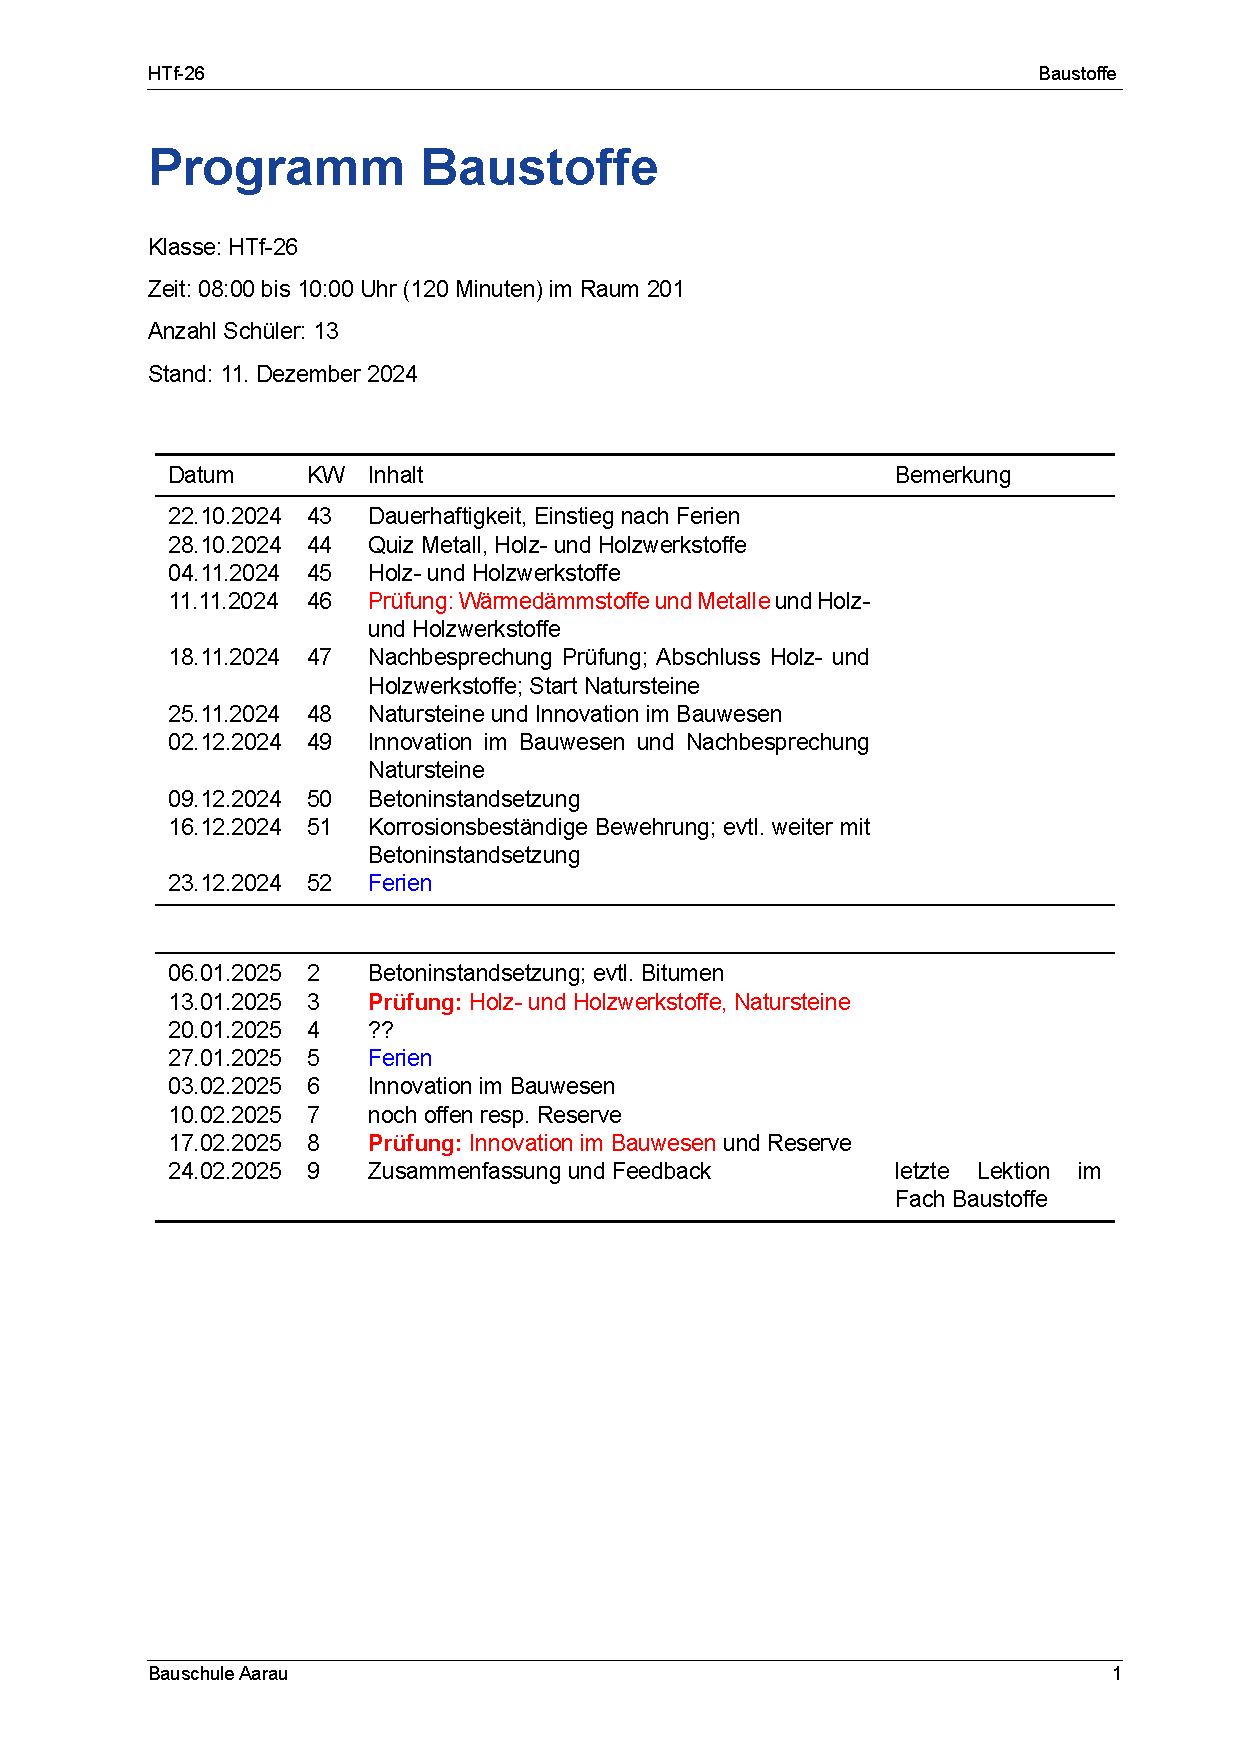
\includepdf[pages=-]{../../HTf-26/Programm/Programm_HTf-26.pdf}
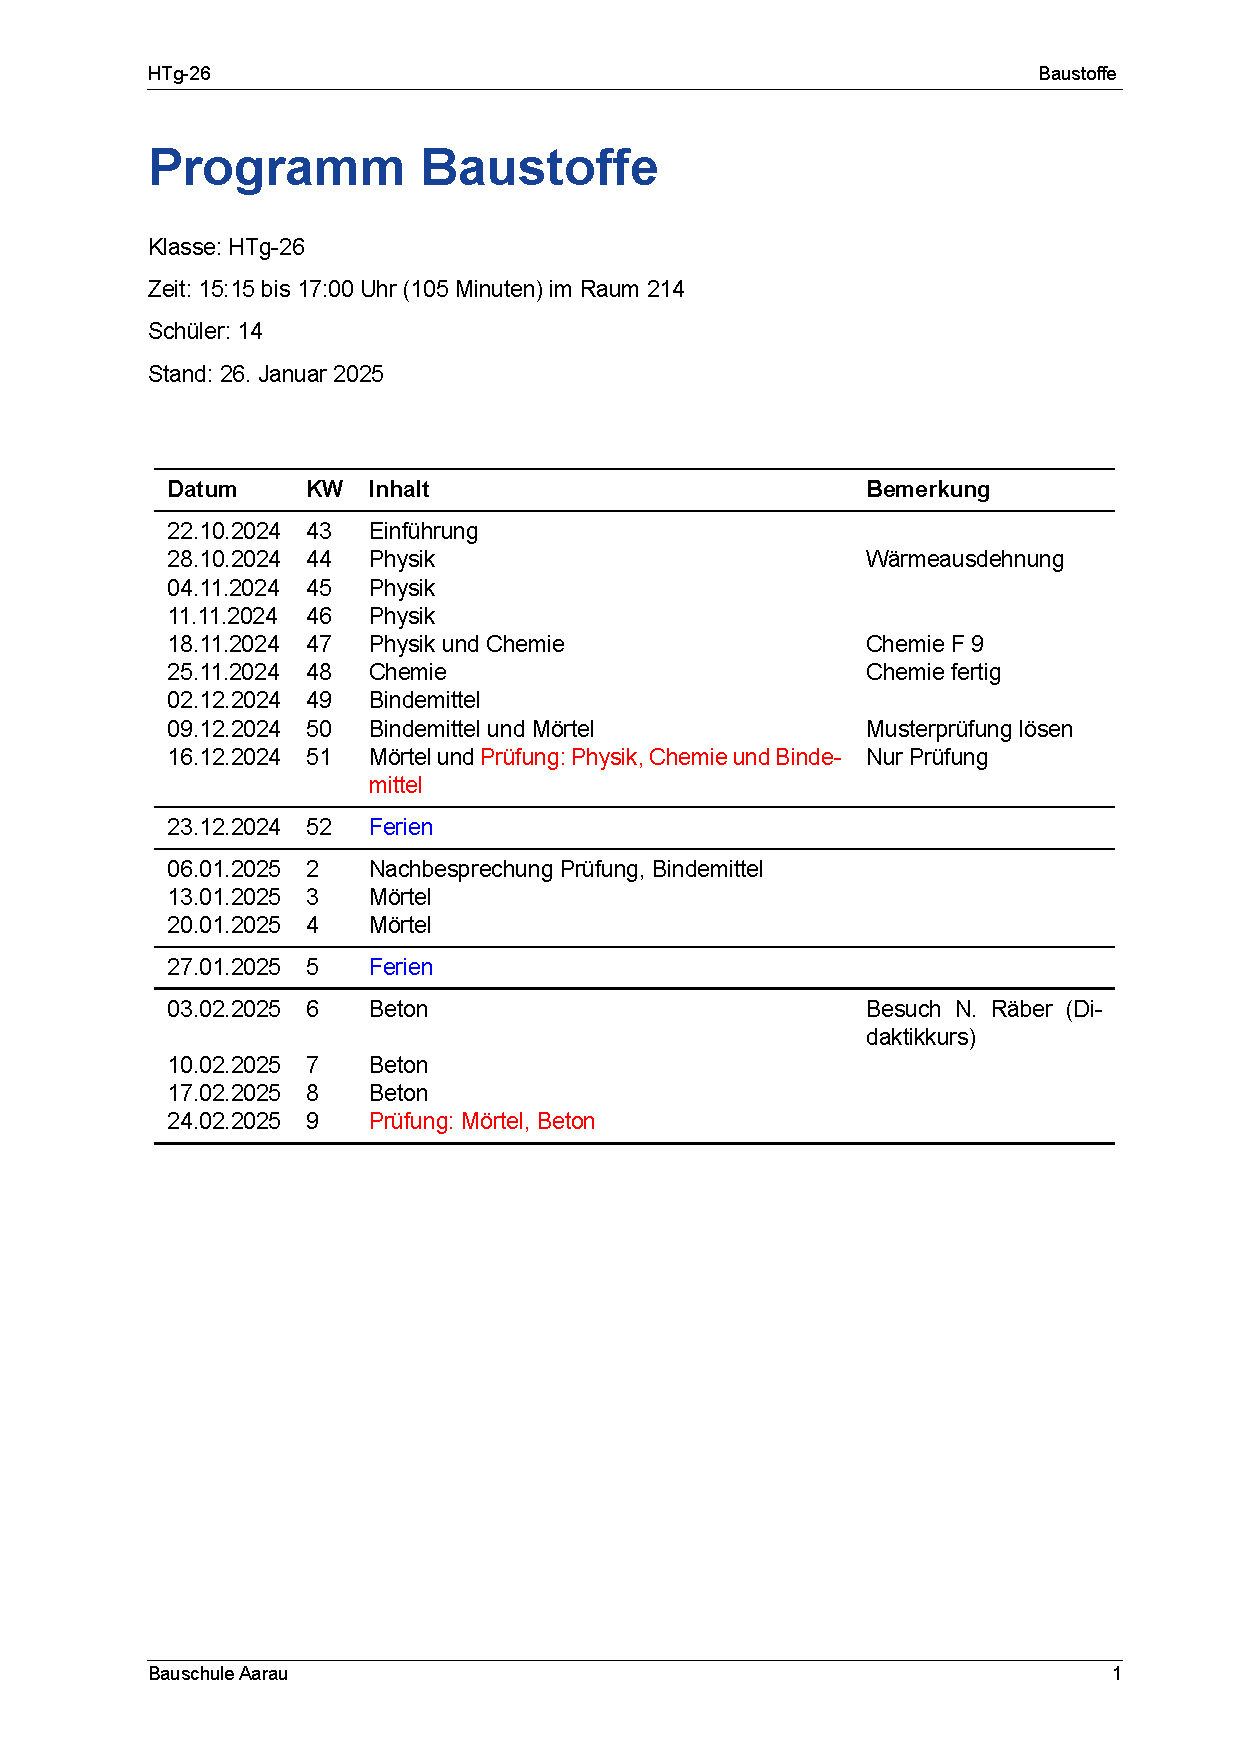
\includepdf[pages=-]{/Users/patricpf/Documents/repos/Bauschule-Baustoffe/HTg-26/Programm/Programm_HTg-26.pdf}



%\section*{Lernziele}
%\addcontentsline{toc}{subsection}{Lernziele}

%Beispiel von Lernzielen einer Prüfung:
%\clearpage
%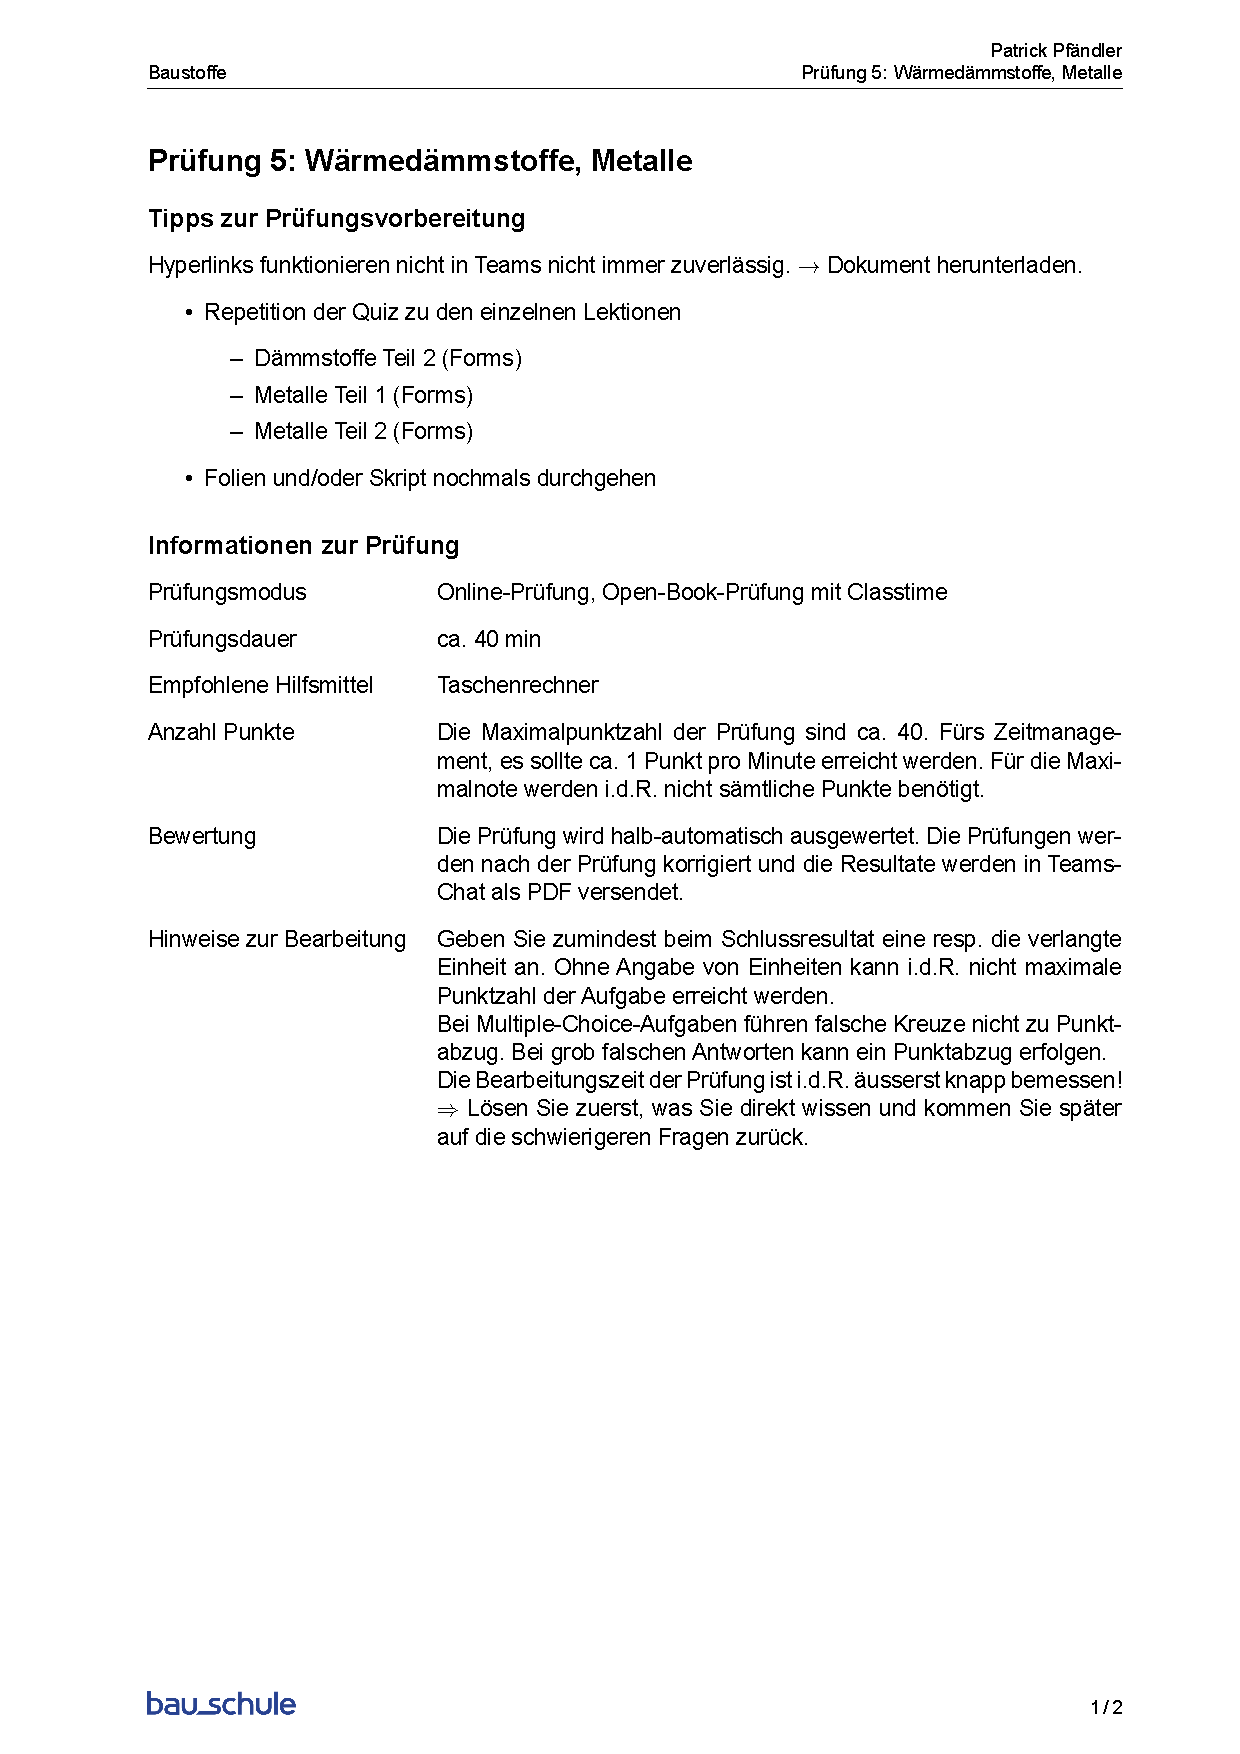
\includepdf[pages=-]{../..//HTf-26/WDS_Metall/Pr5_WDS_Metalle_Lernziele.pdf}


%\clearpage
%\subsection{Folien für die Lektion}
%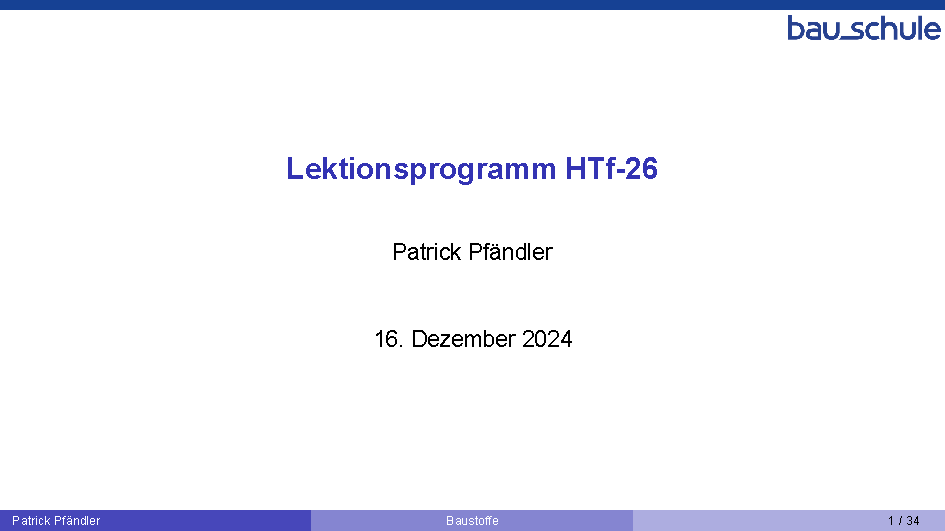
\includepdf[pages=-]{../../HTf-26/KW_51_Programm.pdf}

\end{document}